\chapter{संश्लेषण की रणनीति और हरित रसायन}\label{ch:g12:synthesis-strategy}

एक ही दर्दनाशक, आइबुप्रोफ़ेन, दो तरीकों से बनाया गया है। पुराना
रास्ता छह चरण लेता है, और जो प्रारंभिक सामग्री वह ख़रीदता है, उसके हर सौ किलोग्राम में से
साठ अपशिष्ट बन जाते हैं। नया रास्ता तीन
चरण लेता है, और ख़रीदा गया लगभग हर \omterm{def:g7:atoms-and-molecules:atom}{परमाणु} रख लेता है। दोनों गोली में वही सफ़ेद
चूर्ण देते हैं; उनका अंतर योजना में है। किसी \omterm{def:g10:synthesis-yield:synthesis}{संश्लेषण} की योजना बनाने वाला
रसायनज्ञ चार प्रश्न पूछता है: तेज़ी से कैसे चलें, अधिक कैसे पाएँ, \omterm{def:g7:atoms-and-molecules:molecule}{अणु} के
केवल सही भाग को कैसे छुएँ, और कम से कम कैसे गँवाएँ।

\begin{recall}
\omterm{def:g10:synthesis-yield:synthesis}{संश्लेषण}: अभिक्रिया, पृथक्करण, शोधन, पहचान; उसकी
\omterm{def:g10:synthesis-yield:yield}{लब्धि} (\cref{ch:g10:synthesis-yield})। \omterm{def:g12:curly-arrows:curly-arrow}{वक्र तीर}, \omterm{def:g12:curly-arrows:categories}{प्रतिस्थापन},
योगज, \omterm{def:g12:curly-arrows:categories}{विलोपन} (\cref{ch:g12:curly-arrows})। \omterm{def:g12:catalysis:catalyst}{उत्प्रेरक} बिना खपे किसी अभिक्रिया को
तेज़ करता है (\cref{ch:g12:catalysis})। \omterm{def:g12:equilibrium:non-total}{अपूर्ण
अभिक्रिया} $Q = K$ पर रुकती है; किसी \omterm{def:g7:chemical-reactions:reactant}{अभिकारक} की अधिकता, या किसी उत्पाद को
हटाना, उसे आगे ले जाता है (\cref{ch:g12:equilibrium})।
\end{recall}

\begin{omfigure}
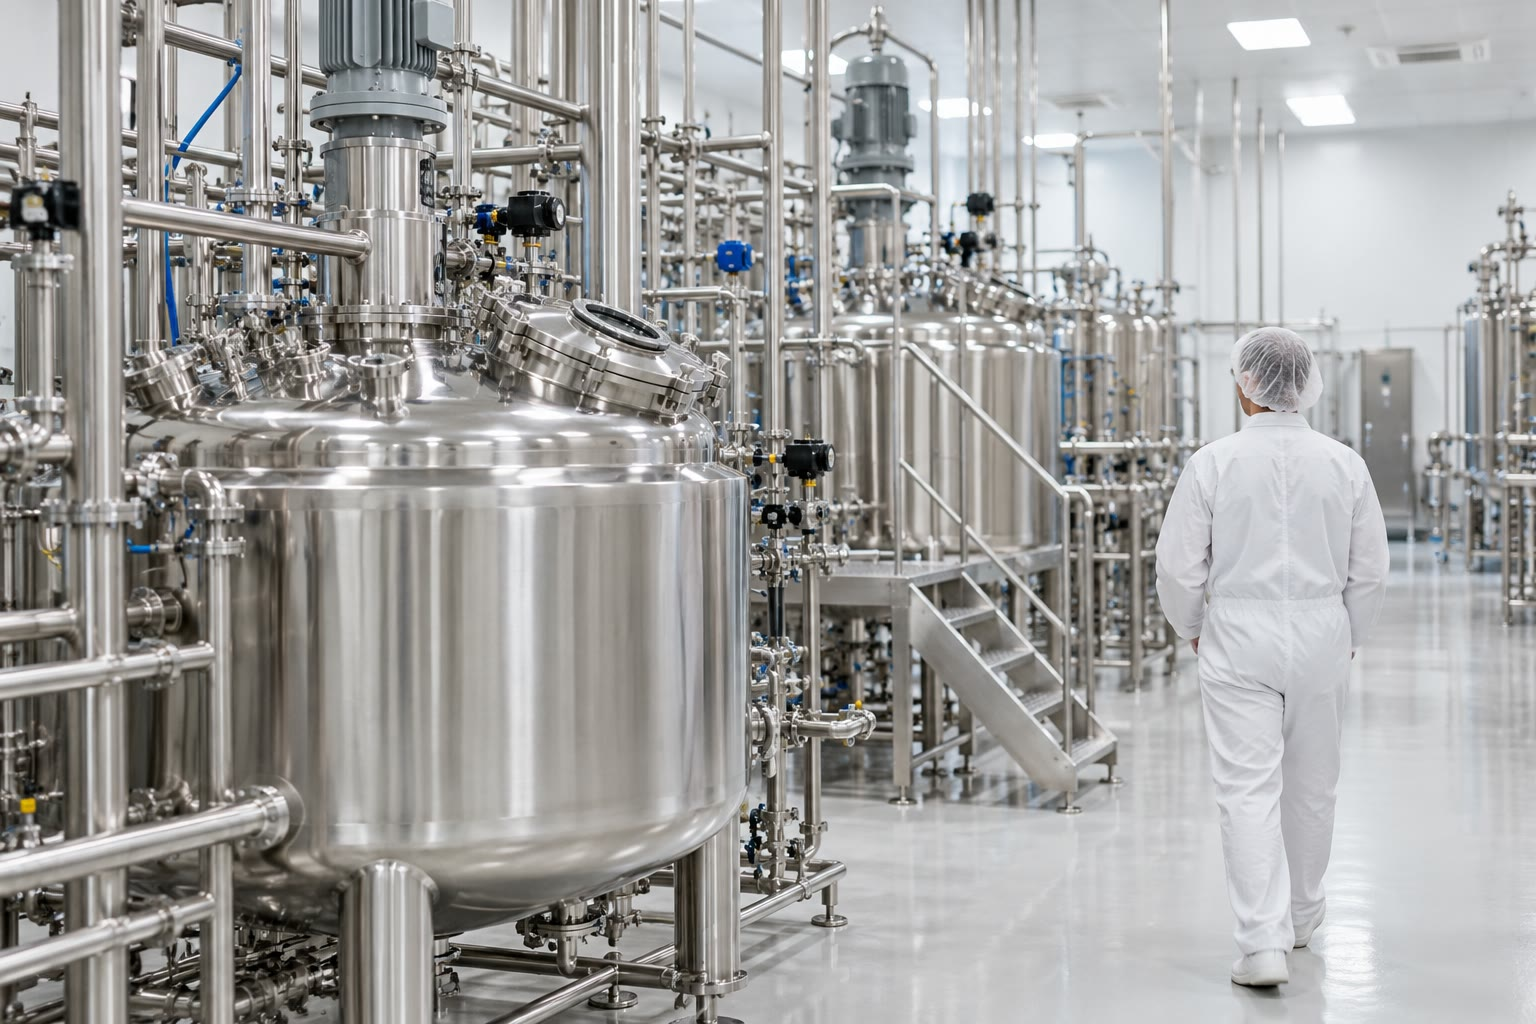
\includegraphics[width=0.48\linewidth]{images/book1/ai/g12-pharma-plant.jpg}

{\small एक औषधि कारख़ाना: \omterm{def:g10:synthesis-yield:synthesis}{संश्लेषण} के रिएक्टर, जिनका पैमाना
टनों तक बढ़ाया गया है।}
\end{omfigure}

\section{संश्लेषण का इष्टतमीकरण}

दो भिन्न चीज़ें सुधारी जा सकती हैं: \emph{दर}, जो तय करती है कि
\omterm{def:g10:synthesis-yield:synthesis}{संश्लेषण} में कितना समय लगता है, और \emph{\omterm{def:g10:synthesis-yield:yield}{लब्धि}}, जो तय करती है कि वह कितना
उत्पाद देता है।

\begin{proposition}[दर और लब्धि के उत्तोलक]\label{prop:g12:synthesis-strategy:levers}
\begin{itemize}
  \item दर ताप के साथ, \omterm{def:g7:chemical-reactions:reactant}{अभिकारकों} की सांद्रताओं के साथ,
        और \omterm{def:g12:catalysis:catalyst}{उत्प्रेरक} के साथ बढ़ती है।
  \item \omterm{def:g10:reaction-progress-table:limiting}{पूर्ण अभिक्रिया} की अंतिम \omterm{def:g10:synthesis-yield:yield}{लब्धि} \omterm{def:g10:reaction-progress-table:limiting}{सीमांत अभिकारक} से
        तय होती है; \omterm{def:g12:equilibrium:non-total}{अपूर्ण अभिक्रिया} की \omterm{def:g10:synthesis-yield:yield}{लब्धि} किसी एक \omterm{def:g7:chemical-reactions:reactant}{अभिकारक} की
        अधिकता से, या बनते ही किसी उत्पाद को हटाने से, बढ़ती है।
        \omterm{def:g12:catalysis:catalyst}{उत्प्रेरक} उसे नहीं बदलता: वह केवल निकाय को उसी \omterm{def:g10:reaction-progress-table:system}{अंतिम अवस्था} तक
        जल्दी पहुँचाता है।
\end{itemize}
\end{proposition}

\begin{proof}
पहला बिंदु \cref{ch:g12:reaction-rates,ch:g12:catalysis} के \omterm{def:g12:reaction-rates:kinetic-factor}{गतिक कारकों}
को एकत्र करता है। दूसरा \omterm{def:g12:equilibrium:non-total}{अपूर्ण अभिक्रिया} के अंत में
$Q = K$ से निकलता है: कोई \omterm{def:g7:chemical-reactions:reactant}{अभिकारक} मिलाना या कोई उत्पाद हटाना
$Q < K$ कर देता है, और अभिक्रिया आगे बढ़ती है।
\end{proof}

\begin{example}[जल-पाश के साथ एस्टरीकरण]\label{ex:g12:synthesis-strategy:trap}
एथेनोइक अम्ल और एथेनॉल, हर एक का एक \omterm{def:g10:the-mole:amount}{मोल}, साम्य पर केवल
\qty{67}{\percent} \omterm{def:g11:functional-groups:carboxylic-acid}{एस्टर} देते हैं। यदि \omterm{def:g6:pure-substances-and-mixtures:mixture}{मिश्रण} को पानी से न मिलने वाले \omterm{def:g6:solutions-and-solubility:solute}{विलायक} में,
\omterm{def:g12:catalysis:catalyst}{उत्प्रेरक} के रूप में थोड़े-से अम्ल के साथ, \omterm{def:g10:synthesis-yield:reflux}{पश्चवाह तापन} किया जाए,
तो वाष्प एक पार्श्व नली में संघनित होती है, जो एक \emph{जल-पाश} है:
अधिक घना पानी तली में बैठकर वहीं रहता है, जबकि
\omterm{def:g6:solutions-and-solubility:solute}{विलायक} वापस फ़्लास्क में बह जाता है। पानी बनते ही अभिक्रिया से
निकल जाता है, $Q$, $K$ से नीचे रहता है, और एस्टरीकरण लगभग
पूर्णता तक पहुँचता है। तापन दर देता है, \omterm{def:g12:catalysis:catalyst}{उत्प्रेरक} और अधिक दर, पाश
\omterm{def:g10:synthesis-yield:yield}{लब्धि}।
\end{example}

\begin{omfigure}
\begin{tikzpicture}[font=\small, scale=0.8]
  \pic[transform shape] at (0,0) {hotplate};
  \pic[transform shape] at (0,0) {rbflask={0.55}{orange!20}};
  % the trap: water at the bottom, solvent above, up to the arm
  \fill[cyan!60!blue!40] (1.0,1.75) arc[start angle=180, end angle=360, radius=0.15] -- (1.3,2.3) -- (1.0,2.3) -- cycle;
  \fill[yellow!35] (1.0,2.3) rectangle (1.3,3.25);
  \draw[om glass] (-0.2,3.0) -- (-0.2,3.75) -- (0.2,3.75) -- (0.2,3.55) -- (1.0,3.55) -- (1.0,4.0);
  \draw[om glass] (0.2,3.0) -- (0.2,3.25) -- (1.0,3.25) -- (1.0,1.75) arc[start angle=180, end angle=360, radius=0.15] -- (1.3,4.0);
  \pic[transform shape] at (1.15,4.0) {condenser};
  \draw[omProp, thick, <-] (1.35,2.0) -- (2.6,1.7) node[right, text=black, align=left] {पानी तली में\\ एकत्र होता है};
  \draw[omProp, thick, <-] (1.35,2.9) -- (2.6,3.1) node[right, text=black, align=left] {विलायक छलककर\\ फ़्लास्क में लौटता है};
  \draw[omProp, thick, <-] (-0.6,0.6) -- (-1.7,1.1) node[left, text=black, align=right] {अम्ल, ऐल्कोहॉल,\\ उत्प्रेरक, विलायक};
\end{tikzpicture}

{\small \omterm{def:g10:synthesis-yield:reflux}{पश्चवाह तापन} वाले फ़्लास्क पर एक जल-पाश: बना हुआ पानी
संघनित होते ही अभिक्रिया से हटा दिया जाता है।}
\end{omfigure}

\section{वरणात्मकता}

किसी वास्तविक \omterm{def:g7:atoms-and-molecules:molecule}{अणु} में अक्सर कई \omterm{def:g11:functional-groups:functional-group}{क्रियात्मक समूह} होते हैं। जो \omterm{def:g7:identifying-substances:characteristic-test}{अभिकर्मक}
उन सब पर आक्रमण करे, वह \omterm{def:g6:pure-substances-and-mixtures:mixture}{मिश्रण} देता है; अच्छा \omterm{def:g10:synthesis-yield:synthesis}{संश्लेषण} ऐसा \omterm{def:g7:identifying-substances:characteristic-test}{अभिकर्मक} इस्तेमाल करता है जो
केवल बदले जाने वाले समूह पर आक्रमण करे।

\begin{definition}[रसायन-वरणात्मक अभिक्रिया]\label{def:g12:synthesis-strategy:chemoselective}
कोई अभिक्रिया \emph{रसायन-वरणात्मक}\index{रसायन-वरणात्मक अभिक्रिया} है जब
कई \omterm{def:g11:functional-groups:functional-group}{क्रियात्मक समूहों} वाले \omterm{def:g7:atoms-and-molecules:molecule}{अणु} पर उसका \omterm{def:g7:identifying-substances:characteristic-test}{अभिकर्मक}
एक समूह को रूपांतरित करता है और दूसरों को अपरिवर्तित छोड़ देता है।
\end{definition}

\begin{example}[चुनने वाला एक अपचायक]\label{ex:g12:synthesis-strategy:nabh4}
सोडियम बोरोहाइड्राइड, \ce{NaBH4}, \omterm{def:g11:functional-groups:carbonyl}{ऐल्डिहाइडों} और \omterm{def:g11:functional-groups:carbonyl}{कीटोनों} के कार्बोनिल समूह को
\omterm{def:g11:functional-groups:alcohol}{ऐल्कोहॉल} समूह में अपचयित करता है, पर \omterm{def:g11:functional-groups:carboxylic-acid}{एस्टरों} को छूता नहीं। जिस
\omterm{def:g7:atoms-and-molecules:molecule}{अणु} में एक \omterm{def:g11:functional-groups:carbonyl}{कीटोन} और एक \omterm{def:g11:functional-groups:carboxylic-acid}{एस्टर} हो, उसमें केवल \omterm{def:g11:functional-groups:carbonyl}{कीटोन} बदलता है:
\[
  \ce{CH3-CO-CH2-CH2-CO-O-CH3}
  \;\xrightarrow{\ \ce{NaBH4}\ }\;
  \ce{CH3-CH(OH)-CH2-CH2-CO-O-CH3} .
\]
अधिक प्रबल \omterm{def:g11:redox:oxidant}{अपचायक}, लिथियम ऐलुमिनियम हाइड्राइड \ce{LiAlH4}, दोनों
समूहों को अपचयित कर देता: यहाँ वह \omterm{def:g12:synthesis-strategy:chemoselective}{रसायन-वरणात्मक} नहीं है।
\end{example}

\begin{remark}[वरणात्मकता के कई प्रकार]\label{rem:g12:synthesis-strategy:kinds}
रसायन-वरणात्मकता समूहों के बीच चुनती है। कोई अभिक्रिया
एक ही समूह की दो स्थितियों के बीच भी चुन सकती है, या उत्पाद के दो \omterm{def:g12:stereochemistry:stereoisomer}{त्रिविम समावयवियों}
के बीच, जैसा \cref{ch:g12:catalysis} के \omterm{def:g12:catalysis:enzyme}{एंज़ाइमों} और
\cref{ch:g12:stereochemistry} के \omterm{def:g12:stereochemistry:chiral}{किरैल} \omterm{def:g7:atoms-and-molecules:molecule}{अणुओं} ने दिखाया। हर प्रकार का अध्ययन
विश्वविद्यालय के खंडों में होता है।
\end{remark}

\section{रक्षी समूह}

जब कोई \omterm{def:g7:identifying-substances:characteristic-test}{अभिकर्मक} पर्याप्त वरणात्मक न हो, तो रसायनज्ञ उस समूह को छिपा देता है जिसे
अभिक्रिया नहीं करनी चाहिए, अभिक्रिया करता है, और फिर समूह को दोबारा खोल देता है।

\begin{definition}[रक्षी समूह]\label{def:g12:synthesis-strategy:protecting-group}
\emph{रक्षी समूह}\index{रक्षी समूह} वह समूह है जो किसी
\omterm{def:g11:functional-groups:functional-group}{क्रियात्मक समूह} से जोड़ा जाता है ताकि वह \omterm{def:g10:synthesis-yield:synthesis}{संश्लेषण} के एक या अधिक चरणों के दौरान
अभिक्रिया न करे, और बाद में हटा दिया जाता है ताकि मूल समूह वापस मिल जाए। ये
तीन संक्रियाएँ \emph{रक्षण}, \emph{अभिक्रिया} और
\emph{विरक्षण} हैं।
\end{definition}

\begin{method}[रक्षण की योजना]\label{met:g12:synthesis-strategy:plan}
\begin{enumerate}
  \item हर \omterm{def:g7:chemical-reactions:reactant}{अभिकारक} के समूहों और बनाए जाने वाले एक आबंध की सूची बनाइए।
  \item हर उस दूसरे समूह को चिह्नित कीजिए जिस पर उस चरण का \omterm{def:g7:identifying-substances:characteristic-test}{अभिकर्मक} भी
        आक्रमण कर सकता है।
  \item उनमें से हर एक की ऐसे समूह से रक्षा कीजिए जो अभिक्रिया की
        परिस्थितियाँ झेल सके और ऐसी सौम्य परिस्थितियों में हटाया जा सके जो
        नए आबंध को अक्षुण्ण छोड़ दें।
  \item लागत गिनिए: हर रक्षण दो चरण जोड़ता है, रक्षण और
        विरक्षण, और समग्र \omterm{def:g10:synthesis-yield:yield}{लब्धि} घटाता है।
\end{enumerate}
\end{method}

\begin{example}[चार नहीं, एक डाइपेप्टाइड बनाना]\label{ex:g12:synthesis-strategy:dipeptide}
ग्लाइसीन, जिसका सूत्र \ce{H2N-CH2-COOH} है, और ऐलानीन, जिसका सूत्र \ce{H2N-CH(CH3)-COOH} है, दोनों में
एक \omterm{def:g11:functional-groups:amine}{ऐमीन} समूह और एक अम्ल समूह है। ग्लाइसीन के अम्ल और
ऐलानीन के \omterm{def:g11:functional-groups:amine}{ऐमीन} के बीच \omterm{def:g11:functional-groups:amine}{ऐमाइड} आबंध डाइपेप्टाइड Gly--Ala देता है। सीधे
मिलाने पर दोनों ऐमीनो अम्ल चार डाइपेप्टाइड देते हैं, Gly--Ala, Ala--Gly,
Gly--Gly और Ala--Ala, एक ऐसे \omterm{def:g6:pure-substances-and-mixtures:mixture}{मिश्रण} में जिसे अलग करना कठिन है। योजना:
\begin{enumerate}
  \item ग्लाइसीन के \omterm{def:g11:functional-groups:amine}{ऐमीन} की रक्षा \ce{Z} लिखे जाने वाले एक समूह से कीजिए, और
        ऐलानीन के अम्ल की उसके मेथिल \omterm{def:g11:functional-groups:carboxylic-acid}{एस्टर} के रूप में;
  \item \omterm{def:g11:functional-groups:amine}{ऐमाइड} आबंध बनाइए: केवल एक अम्ल समूह और एक \omterm{def:g11:functional-groups:amine}{ऐमीन} समूह
        मुक्त बचे हैं;
  \item दोनों \omterm{def:g12:synthesis-strategy:protecting-group}{रक्षी समूह} हटाइए।
\end{enumerate}
\end{example}

\begin{omfigure}
\begin{tikzpicture}[font=\small, node distance=0.55cm,
    box/.style={draw=omDef, rounded corners=2pt, fill=omDef!6, align=center, inner sep=4pt}]
  \node[box] (a) {\ce{H2N-CH2-COOH}\\ \ce{H2N-CH(CH3)-COOH}};
  \node[box, below=of a] (b) {\ce{Z-NH-CH2-COOH}\\ \ce{H2N-CH(CH3)-CO-O-CH3}};
  \node[box, below=of b] (c) {\ce{Z-NH-CH2-CO-NH-CH(CH3)-CO-O-CH3}};
  \node[box, below=of c] (d) {\ce{H2N-CH2-CO-NH-CH(CH3)-COOH}};
  \draw[->, thick, omProp] (a) -- node[right, xshift=3pt, text=black] {1. रक्षण} (b);
  \draw[->, thick, omProp] (b) -- node[right, xshift=3pt, text=black] {2. अभिक्रिया: ऐमाइड आबंध} (c);
  \draw[->, thick, omProp] (c) -- node[right, xshift=3pt, text=black] {3. विरक्षण} (d);
  \node[anchor=east, font=\footnotesize, text=black!70] at ([xshift=-6pt]a.west) {ग्लाइसीन, ऐलानीन};
  \node[anchor=east, font=\footnotesize, text=black!70] at ([xshift=-6pt]d.west) {Gly--Ala};
\end{tikzpicture}

{\small रक्षण, अभिक्रिया, विरक्षण: केवल वही \omterm{def:g11:functional-groups:amine}{ऐमाइड} आबंध बन सकता है
जो चाहिए।}
\end{omfigure}

\section{परमाणु मितव्ययिता}

\qty{100}{\percent} की \omterm{def:g10:synthesis-yield:yield}{लब्धि} बताती है कि \omterm{def:g10:reaction-progress-table:limiting}{सीमांत अभिकारक} का हर \omterm{def:g7:atoms-and-molecules:molecule}{अणु}
उत्पाद बन गया। यह नहीं बताती कि ख़रीदे गए \omterm{def:g7:atoms-and-molecules:atom}{परमाणुओं} में से कितने
उत्पाद में पहुँचे: समीकरण के दूसरे उत्पाद, कितने भी
शुद्ध हों, अपशिष्ट हैं, जब तक कोई उनका उपयोग न कर सके।

\begin{definition}[परमाणु मितव्ययिता]\label{def:g12:synthesis-strategy:atom-economy}
किसी \omterm{def:g10:synthesis-yield:synthesis}{संश्लेषण} की \emph{परमाणु मितव्ययिता}\index{परमाणु मितव्ययिता}
\omterm{def:g7:chemical-reactions:reactant}{अभिकारकों} के द्रव्यमान का, \omterm{def:g8:balanced-equations:equation}{संतुलित समीकरण} के अनुपातों में लेकर, वह
अंश है जो वांछित उत्पाद में पहुँचता है।
\end{definition}

\begin{proposition}[समीकरण से परमाणु मितव्ययिता]\label{prop:g12:synthesis-strategy:atom-economy}
\omterm{def:g8:balanced-equations:equation}{संतुलित समीकरण} $a_1\,\ce{R1} + a_2\,\ce{R2} + \cdots \rightarrow
p\,\ce{P} + \text{अन्य उत्पाद}$ के लिए,
\[
  \text{परमाणु मितव्ययिता} =
  \frac{p\,M(\ce{P})}{a_1 M(\ce{R1}) + a_2 M(\ce{R2}) + \cdots}
  \times 100\,\% .
\]
\end{proposition}

\begin{proof}
अभिक्रिया के $x$ \omterm{def:g10:the-mole:amount}{मोल} के लिए, खपे \omterm{def:g7:chemical-reactions:reactant}{अभिकारकों} का द्रव्यमान
$x\,(a_1 M(\ce{R1}) + \cdots)$ है और बने वांछित उत्पाद का द्रव्यमान
$x\,p\,M(\ce{P})$; उनका अनुपात $x$ पर निर्भर नहीं करता।
\end{proof}

\begin{method}[परमाणु मितव्ययिता निकालना]\label{met:g12:synthesis-strategy:atom-economy}
\begin{enumerate}
  \item \omterm{def:g8:balanced-equations:equation}{संतुलित समीकरण} लिखिए; कई चरणों वाले रास्ते के लिए चरणों को
        इस तरह जोड़िए कि हर मध्यवर्ती कट जाए।
  \item हर \omterm{def:g7:chemical-reactions:reactant}{अभिकारक} और वांछित उत्पाद का \omterm{def:g10:the-mole:molar-mass}{मोलर द्रव्यमान}
        निकालिए।
  \item \omterm{def:g8:balanced-equations:coefficient}{रससमीकरणमितीय गुणांकों} के साथ सूत्र लागू कीजिए।
  \item प्रति किलोग्राम उत्पाद अपशिष्ट
        $(100 - \text{परमाणु मितव्ययिता})/\text{परमाणु मितव्ययिता}$ किलोग्राम है।
\end{enumerate}
\end{method}

\begin{example}[योगज बनाम प्रतिस्थापन]\label{ex:g12:synthesis-strategy:compare}
% ledger: aw:C, aw:H, aw:Br, aw:Na, aw:O
एथीन से ब्रोमोएथेन, \ce{C2H4 + HBr -> C2H5Br}: हर \omterm{def:g7:atoms-and-molecules:atom}{परमाणु}
उत्पाद में पहुँचता है, \omterm{def:g12:synthesis-strategy:atom-economy}{परमाणु मितव्ययिता} $108.9/(28.0 + 80.9) = \qty{100}{\percent}$।
ब्रोमोएथेन से एथेनॉल, \ce{C2H5Br + NaOH -> C2H5OH + NaBr}:
\omterm{def:g12:synthesis-strategy:atom-economy}{परमाणु मितव्ययिता} $46.0/(108.9 + 40.0) = \qty{30.9}{\percent}$ है; प्रति
किलोग्राम एथेनॉल \qty{2.2}{kg} सोडियम ब्रोमाइड। \omterm{def:g12:curly-arrows:categories}{योगज अभिक्रिया} की
\omterm{def:g12:synthesis-strategy:atom-economy}{परमाणु मितव्ययिता} सदा \qty{100}{\percent} होती है; \omterm{def:g12:curly-arrows:categories}{प्रतिस्थापन} या
\omterm{def:g12:curly-arrows:categories}{विलोपन} की कभी नहीं।
\end{example}

\begin{omfigure}
\begin{tikzpicture}
\begin{axis}[width=0.8\linewidth, height=5.2cm, ybar, bar width=16pt,
    ymin=0, ymax=112, ylabel={परमाणु मितव्ययिता (\%)},
    xtick={1,2,3,4,5}, xticklabels={योगज, एस्टरीकरण, आइबुप्रोफ़ेन (3 चरण), आइबुप्रोफ़ेन (6 चरण), प्रतिस्थापन},
    xticklabel style={font=\footnotesize, align=center, text width=2.1cm},
    nodes near coords, nodes near coords style={font=\footnotesize},
    enlarge x limits=0.12, axis lines*=left, ymajorgrids, grid style={black!12}]
  \addplot[fill=omDef!55, draw=omDef] table[x=i, y=AE] {figdata/out/grade-12-synthesis-strategy.dat};
\end{axis}
\end{tikzpicture}

{\small समीकरणों से निकाली गई \omterm{def:g12:synthesis-strategy:atom-economy}{परमाणु मितव्ययिताएँ}: हाइड्रोजन
ब्रोमाइड के साथ एथीन, एथेनॉल के साथ एथेनोइक अम्ल, आइबुप्रोफ़ेन के दोनों रास्ते, और
सोडियम हाइड्रॉक्साइड के साथ ब्रोमोएथेन।}
\end{omfigure}

\section{हरित रसायन}

\begin{definition}[हरित रसायन]\label{def:g12:synthesis-strategy:green-chemistry}
\emph{हरित रसायन}\index{हरित रसायन} ऐसे रासायनिक
उत्पादों और प्रक्रमों की अभिकल्पना है जो ख़तरनाक पदार्थों के उपयोग और
उत्पादन को घटाते या समाप्त करते हैं, प्रारंभिक
सामग्री के चयन से लेकर उपयोग के बाद उत्पाद की नियति तक।
\end{definition}

बारह सिद्धांत इस दृष्टिकोण का सार हैं; हर एक किसी प्रक्रम से पूछा जाने वाला
एक प्रश्न है।
% ledger: green:12
\begin{enumerate}
  \item अपशिष्ट का उपचार करने के बजाय उसे रोकिए।
  \item \omterm{def:g12:synthesis-strategy:atom-economy}{परमाणु मितव्ययिता} अधिकतम कीजिए।
  \item कम ख़तरनाक \omterm{def:g10:synthesis-yield:synthesis}{संश्लेषणों} की अभिकल्पना कीजिए।
  \item अधिक सुरक्षित रसायनों और उत्पादों की अभिकल्पना कीजिए।
  \item अधिक सुरक्षित \omterm{def:g6:solutions-and-solubility:solute}{विलायक} और अभिक्रिया परिस्थितियाँ इस्तेमाल कीजिए।
  \item ऊर्जा दक्षता बढ़ाइए: कमरे के ताप और दाब के निकट
        काम कीजिए।
  \item नवीकरणीय \omterm{def:g5:raw-materials-and-recycling:raw-material}{कच्चा माल} इस्तेमाल कीजिए।
  \item रासायनिक व्युत्पन्नों, जैसे \omterm{def:g12:synthesis-strategy:protecting-group}{रक्षी समूहों}, से बचिए।
  \item रससमीकरणमितीय \omterm{def:g7:identifying-substances:characteristic-test}{अभिकर्मकों} के बजाय \omterm{def:g12:catalysis:catalyst}{उत्प्रेरक} इस्तेमाल कीजिए।
  \item ऐसे उत्पादों की अभिकल्पना कीजिए जो उपयोग के बाद विघटित हो जाएँ।
  \item प्रदूषण रोकने के लिए वास्तविक समय में विश्लेषण कीजिए।
  \item दुर्घटनाओं की संभावना न्यूनतम कीजिए।
\end{enumerate}

\begin{remark}[सिद्धांत, नियम नहीं]\label{rem:g12:synthesis-strategy:principles}
ये सिद्धांत अक्सर विपरीत दिशाओं में खींचते हैं: \omterm{def:g12:synthesis-strategy:protecting-group}{रक्षी समूह}
सिद्धांत 8 तोड़ता है पर पूरे \omterm{def:g10:synthesis-yield:synthesis}{संश्लेषण} को बचा सकता है; ऊर्जा बचाने वाले \omterm{def:g12:catalysis:catalyst}{उत्प्रेरक} में
कोई दुर्लभ \omterm{def:g9:periodic-table-first-look:metal}{धातु} हो सकती है। किसी प्रक्रम का मूल्यांकन करने का अर्थ है उन्हें तौलना,
जहाँ तक संभव हो संख्याओं के साथ: \omterm{def:g12:synthesis-strategy:atom-economy}{परमाणु मितव्ययिता}, \omterm{def:g10:synthesis-yield:yield}{लब्धि}, अपशिष्ट का द्रव्यमान,
ऊर्जा।
\end{remark}

\begin{history}[हरित रसायन, 1998]
% ledger: green:book-1998, ibu:bhc-commercial
1998 में रसायनज्ञ पॉल अनास्तास और जॉन वॉर्नर ने एक पुस्तक प्रकाशित की,
\emph{\omterm{def:g12:synthesis-strategy:green-chemistry}{हरित रसायन}: सिद्धांत और व्यवहार}, जिसने बारह
सिद्धांत प्रस्तुत किए। एक वर्ष पहले, अधिक हरित \omterm{def:g10:synthesis-yield:synthesis}{संश्लेषणों} के लिए एक सरकारी पुरस्कार
आइबुप्रोफ़ेन के तीन-चरण वाले रास्ते को मिला था, जो 1992 से औद्योगिक पैमाने पर
चल रहा था। तब से ये सिद्धांत रसायनज्ञों को उनके पेशे के
एक भाग के रूप में पढ़ाए जाते हैं।
\end{history}

\begin{example}[आइबुप्रोफ़ेन तक दो रास्ते]\label{ex:g12:synthesis-strategy:ibuprofen}
% ledger: ibu:boots-steps, ibu:bhc-steps, ibu:boots-ae, ibu:bhc-ae, ibu:bhc-ae-recovered
आइबुप्रोफ़ेन, \ce{C13H18O2}, हाइड्रोकार्बन
\ce{C10H14} (आइसोब्यूटिलबेंज़ीन) से बनाया जाता है। पुराना रास्ता छह चरण इस्तेमाल करता है और
हर एक में \omterm{def:g7:identifying-substances:characteristic-test}{अभिकर्मक} की पूरी मात्रा; सब जोड़ने पर उसके \omterm{def:g7:chemical-reactions:reactant}{अभिकारकों} का
\omterm{def:g10:the-mole:molar-mass}{मोलर द्रव्यमान} योग \qty{514.5}{g/mol} है, जबकि आइबुप्रोफ़ेन का
\qty{206.0}{g/mol}: \omterm{def:g12:synthesis-strategy:atom-economy}{परमाणु मितव्ययिता} \qty{40}{\percent}। नया रास्ता तीन
चरण इस्तेमाल करता है, जिनमें से दो उत्प्रेरित हैं, और समग्र समीकरण
\[
  \ce{C10H14 + C4H6O3 + H2 + CO -> C13H18O2 + C2H4O2}
\]
$206.0/266.0 = \qty{77}{\percent}$ देता है। उसका उप-उत्पाद, एथेनोइक अम्ल,
पुनः प्राप्त करके इस्तेमाल किया जाता है: उत्पाद के रूप में गिनने पर \omterm{def:g12:synthesis-strategy:atom-economy}{परमाणु मितव्ययिता}
\qty{99}{\percent} से अधिक हो जाती है।
\end{example}

\begin{omfigure}
\chemfig{[:30]*6(-=(-[:90](-[:150])-[:30](=[:90]O)-[:-30]OH)-=-(-[:-90]-[:-150](-[:150])-[:-90])=)}

\medskip
\begin{tikzpicture}[font=\scriptsize,
    st/.style={draw=omDef, rounded corners=2pt, fill=omDef!6, minimum height=0.8cm, text width=1.15cm, align=center, inner sep=2pt}]
  \foreach \i/\t in {1/ऐसिलन, 2/+ 2 कार्बन, 3/ऐल्डिहाइड, 4/ऑक्सिम, 5/नाइट्राइल, 6/अम्ल}
    \node[st] (o\i) at (1.7*\i,0) {\t};
  \foreach \i/\j in {1/2,2/3,3/4,4/5,5/6} \draw[->, thick] (o\i) -- (o\j);
  \node[anchor=east, align=right, font=\footnotesize] at ([xshift=-4pt]o1.west) {6 चरण\\ \textbf{40 \%}};
  \foreach \i/\t in {1/ऐसिलन, 2/\ce{H2} का योग, 3/\ce{CO} का योग}
    \node[st, fill=omProp!8, draw=omProp] (n\i) at (1.7*\i,-1.4) {\t\\ (उत्प्रेरक)};
  \foreach \i/\j in {1/2,2/3} \draw[->, thick] (n\i) -- (n\j);
  \node[anchor=east, align=right, font=\footnotesize] at ([xshift=-4pt]n1.west) {3 चरण\\ \textbf{77 \%}};
  \node[anchor=west, align=left, font=\footnotesize] at ([xshift=6pt]n3.east) {उप-उत्पाद: एथेनोइक अम्ल, पुनः प्राप्त;\\ उत्पाद के रूप में गिनने पर: 99 \% से अधिक};
\end{tikzpicture}

{\small आइबुप्रोफ़ेन (ऊपर) और उसके दो औद्योगिक रास्ते: पुराना,
छह चरण, और नया, तीन उत्प्रेरित चरण, अपनी \omterm{def:g12:synthesis-strategy:atom-economy}{परमाणु
मितव्ययिताओं} के साथ।}
\end{omfigure}

\begin{example}[अधिक हरित विलायक]\label{ex:g12:synthesis-strategy:solvents}
% ledger: crit:CO2-T, crit:CO2-p
अनेक अभिक्रियाएँ और \omterm{def:g10:chemical-species:extraction}{निष्कर्षण} ऐसे कार्बनिक \omterm{def:g6:solutions-and-solubility:solute}{विलायक} इस्तेमाल करते हैं जो विषैले,
ज्वलनशील या वाष्पशील हैं। पानी सबसे सुरक्षित \omterm{def:g6:solutions-and-solubility:solute}{विलायक} है, जब
\omterm{def:g7:chemical-reactions:reactant}{अभिकारक} उसमें \omterm{def:g2:mixing-and-dissolving:dissolve}{घुलते} हों। कार्बन डाइऑक्साइड एक और बन जाती है:
\qty{31}{\celsius} और \qty{73.8}{bar} से ऊपर वह एक \emph{अतिक्रांतिक
तरल} है, न द्रव न गैस, जो अनेक कार्बनिक \omterm{def:g7:atoms-and-molecules:molecule}{अणुओं} को घोलता है।
उदाहरण के लिए, वह कॉफ़ी के बीजों से कैफ़ीन निकालती है; दाब
हटाने पर वह बस फिर से गैस बन जाती है और उत्पाद में कोई अवशेष नहीं
छोड़ती।
\end{example}

\begin{omfigure}
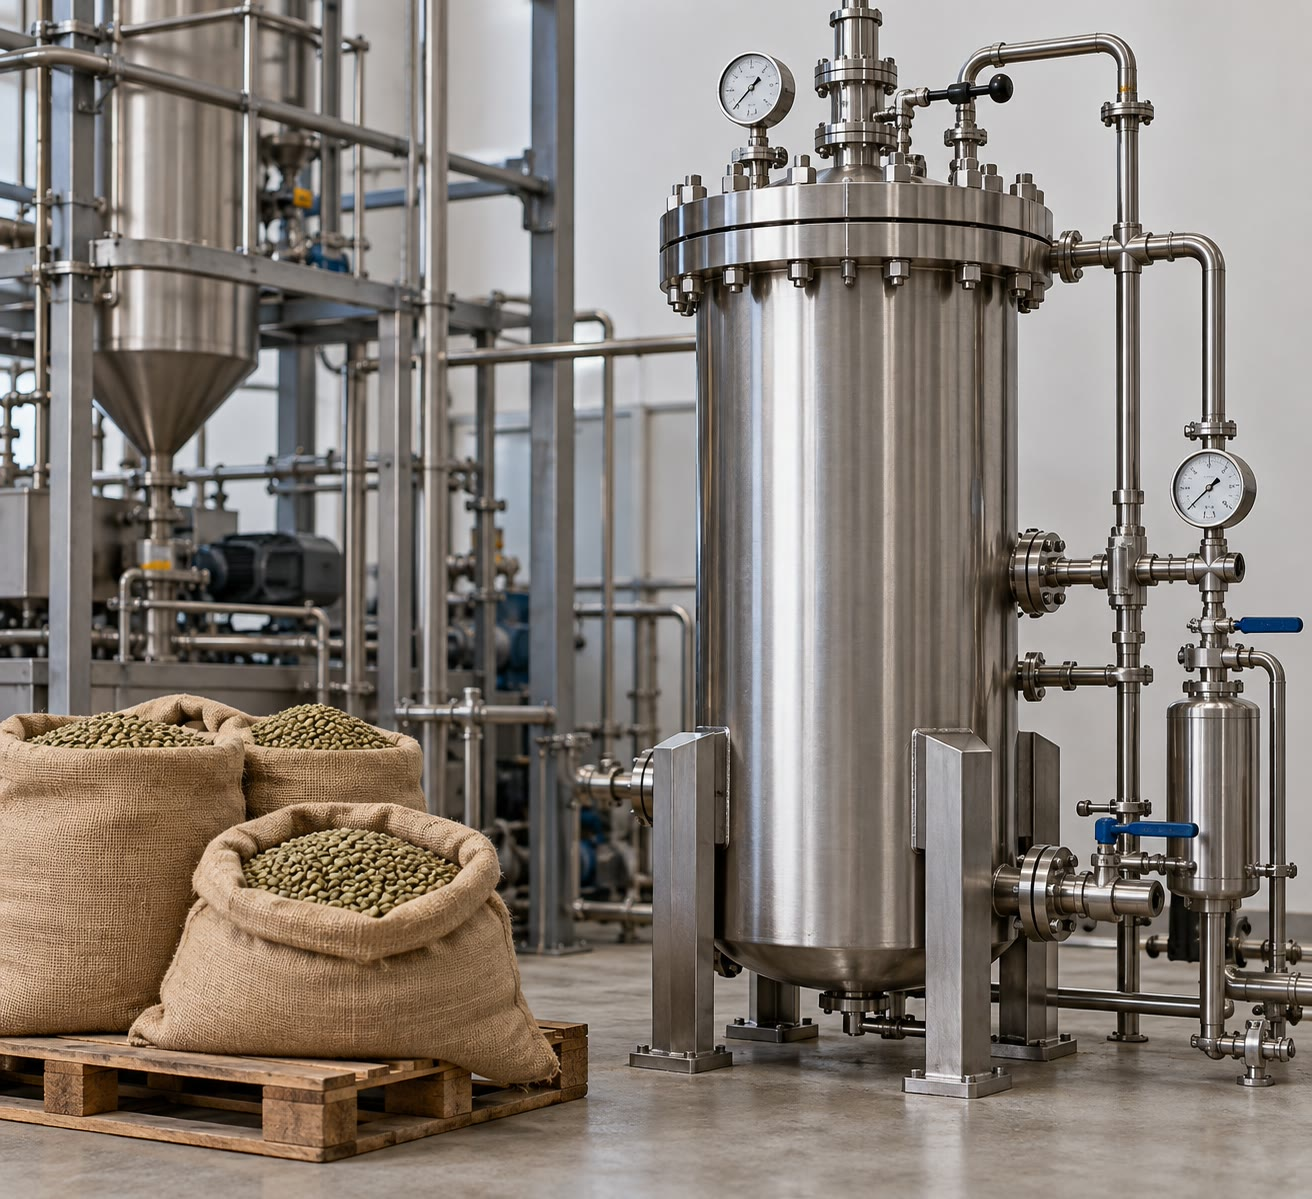
\includegraphics[width=0.45\linewidth,height=6cm,keepaspectratio]{images/book1/ai/g12-scco2-vessel.jpg}

{\small एक उच्च-दाब \omterm{def:g10:chemical-species:extraction}{निष्कर्षण} पात्र, जिसमें अतिक्रांतिक कार्बन
डाइऑक्साइड किसी कार्बनिक \omterm{def:g6:solutions-and-solubility:solute}{विलायक} की जगह लेती है।}
\end{omfigure}

\section{अभ्यास}

\begin{exercise}[$\star$]\label{exo:g12:synthesis-strategy:1}
एथेनॉल एथीन के जलयोजन, \ce{C2H4 + H2O -> C2H5OH}, से
या ग्लूकोज़ के किण्वन, \ce{C6H12O6 -> 2C2H5OH + 2CO2}, से बनाया जा सकता है। हर एक की
\omterm{def:g12:synthesis-strategy:atom-economy}{परमाणु मितव्ययिता} निकालिए।
\end{exercise}

\begin{exercise}[$\star$]\label{exo:g12:synthesis-strategy:2}
इस अध्याय की डाइपेप्टाइड योजना में वह चरण बताइए जिसमें हर
\omterm{def:g12:synthesis-strategy:protecting-group}{रक्षी समूह} लगाया जाता है, और वह चरण जिसमें वह हटाया जाता है।
\end{exercise}

\begin{exercise}[$\star$]\label{exo:g12:synthesis-strategy:3}
एक कारख़ाना अपनी एक अभिक्रिया में क्लोरीनयुक्त \omterm{def:g6:solutions-and-solubility:solute}{विलायक} की जगह पानी इस्तेमाल करने लगता है।
वह \omterm{def:g12:synthesis-strategy:green-chemistry}{हरित रसायन} का कौन-सा सिद्धांत लागू करता है?
\end{exercise}

\begin{exercise}[$\star$]\label{exo:g12:synthesis-strategy:4}
एथेनॉल की अधिकता एस्टरीकरण की \omterm{def:g10:synthesis-yield:yield}{लब्धि} क्यों बढ़ाती है, जबकि
\omterm{def:g12:catalysis:catalyst}{उत्प्रेरक} नहीं बढ़ाता?
\end{exercise}

\begin{exercise}[$\star$]\label{exo:g12:synthesis-strategy:5}
सोडियम बोरोहाइड्राइड \omterm{def:g11:functional-groups:carbonyl}{ऐल्डिहाइडों} और \omterm{def:g11:functional-groups:carbonyl}{कीटोनों} को अपचयित करता है, \omterm{def:g11:functional-groups:carboxylic-acid}{एस्टरों} को नहीं। क्या
मेथिल 4-ऑक्सोपेंटेनोएट (एक \omterm{def:g11:functional-groups:carbonyl}{कीटोन} और एक \omterm{def:g11:functional-groups:carboxylic-acid}{एस्टर}) के साथ उसकी अभिक्रिया
\omterm{def:g12:synthesis-strategy:chemoselective}{रसायन-वरणात्मक} है? कौन-सा समूह बदलता है?
\end{exercise}

\begin{exercise}[$\star\star$]\label{exo:g12:synthesis-strategy:6}
एथेनोइक अम्ल का एक \omterm{def:g10:the-mole:amount}{मोल} और एथेनॉल का एक \omterm{def:g10:the-mole:amount}{मोल} साम्य पर \qty{0.67}{mol}
\omterm{def:g11:functional-groups:carboxylic-acid}{एस्टर} देते हैं। इस मात्रा को बढ़ाने के दो तरीके, और उस तक जल्दी पहुँचने का
एक तरीका प्रस्तावित कीजिए।
\end{exercise}

\begin{exercise}[$\star\star$]\label{exo:g12:synthesis-strategy:7}
मेथिल 4-ऑक्सोपेंटेनोएट, \ce{CH3-CO-CH2-CH2-CO-O-CH3}, को एक बार
सोडियम बोरोहाइड्राइड से, और एक बार लिथियम ऐलुमिनियम
हाइड्राइड की अधिकता से उपचारित किया जाता है, जो \omterm{def:g11:functional-groups:carboxylic-acid}{एस्टर} को दो \omterm{def:g11:functional-groups:alcohol}{ऐल्कोहॉलों} में अपचयित करता है। हर उत्पाद लिखिए।
\end{exercise}

\begin{exercise}[$\star\star$]\label{exo:g12:synthesis-strategy:8}
\omterm{def:g12:synthesis-strategy:atom-economy}{परमाणु मितव्ययिताओं} के दंड आलेख पर कौन-सी अभिक्रियाएँ तीन चौथाई से अधिक
\omterm{def:g7:atoms-and-molecules:atom}{परमाणु} रखती हैं? आइबुप्रोफ़ेन तक तीन-चरण वाला रास्ता छह-चरण वाले से
किस गुणक से बेहतर है?
\end{exercise}

\begin{exercise}[$\star\star$]\label{exo:g12:synthesis-strategy:9}
ऐस्पिरिन \ce{C7H6O3 + C4H6O3 -> C9H8O4 + C2H4O2} से बनाई जाती है। उसकी
\omterm{def:g12:synthesis-strategy:atom-economy}{परमाणु मितव्ययिता} और प्रति किलोग्राम ऐस्पिरिन उप-उत्पाद का द्रव्यमान निकालिए।
\end{exercise}

\begin{exercise}[$\star\star$]\label{exo:g12:synthesis-strategy:10}
किसी \omterm{def:g10:synthesis-yield:synthesis}{संश्लेषण} को खुले फ़्लास्क के बजाय \omterm{def:g10:synthesis-yield:reflux}{पश्चवाह तापन} क्यों किया जाता है?
दर और \omterm{def:g10:synthesis-yield:yield}{लब्धि} में से तापन किसे सुधारता है?
\end{exercise}

\begin{exercise}[$\star\star$]\label{exo:g12:synthesis-strategy:11}
आइबुप्रोफ़ेन के दोनों रास्तों वाले चित्र पर चरण गिनिए और बताइए कि नया
रास्ता \omterm{def:g12:synthesis-strategy:green-chemistry}{हरित रसायन} के कौन-से सिद्धांत लागू करता है। तीन बताइए।
\end{exercise}

\begin{exercise}[$\star\star\star$]\label{exo:g12:synthesis-strategy:12}
एक तीन-चरण \omterm{def:g10:synthesis-yield:synthesis}{संश्लेषण} की \omterm{def:g10:synthesis-yield:yield}{लब्धियाँ} \qty{80}{\percent},
\qty{70}{\percent} और \qty{90}{\percent} हैं। समग्र \omterm{def:g10:synthesis-yield:yield}{लब्धि} निकालिए।
अंतिम उत्पाद का \qty{0.10}{mol} पाने के लिए प्रारंभिक सामग्री की कितनी मात्रा
चाहिए, यदि प्रारंभिक सामग्री का एक \omterm{def:g10:the-mole:amount}{मोल} अधिक से अधिक उत्पाद का एक \omterm{def:g10:the-mole:amount}{मोल}
देता है?
\end{exercise}

\begin{exercise}[$\star\star\star$]\label{exo:g12:synthesis-strategy:13}
डाइपेप्टाइड Ala--Gly (ग्लाइसीन के \omterm{def:g11:functional-groups:amine}{ऐमीन} से आबंधित ऐलानीन का अम्ल) के
\omterm{def:g10:synthesis-yield:synthesis}{संश्लेषण} की योजना बनाइए: आप किन समूहों की रक्षा करते हैं, और योजना में कितने चरण
लगते हैं?
\end{exercise}

\begin{exercise}[$\star\star\star$]\label{exo:g12:synthesis-strategy:14}
एक कंपनी अपने प्रक्रम को ``हरित'' कहती है क्योंकि वह \omterm{def:g12:catalysis:catalyst}{उत्प्रेरक} इस्तेमाल करता है।
प्रक्रम \qty{250}{\celsius} पर एक विषैले \omterm{def:g6:solutions-and-solubility:solute}{विलायक}, बेंज़ीन, में चलता है, और उसकी
\omterm{def:g12:synthesis-strategy:atom-economy}{परमाणु मितव्ययिता} \qty{35}{\percent} है। सिद्धांत-दर-सिद्धांत इस दावे का
मूल्यांकन कीजिए।
\end{exercise}

\begin{exercise}[$\star\star\star$]\label{exo:g12:synthesis-strategy:15}
कॉफ़ी के बीजों से कैफ़ीन या तो डाइक्लोरोमेथेन, एक
वाष्पशील क्लोरीनयुक्त \omterm{def:g6:solutions-and-solubility:solute}{विलायक}, से निकाली जाती है, या लगभग
\qty{40}{\celsius} और \qty{100}{bar} पर अतिक्रांतिक कार्बन डाइऑक्साइड से। समझाइए कि दूसरा
अतिक्रांतिक क्यों है, उसे मज़बूत पात्र की ज़रूरत क्यों है, और पहले की तुलना में उसके
दो लाभ बताइए।
\end{exercise}

\section{समस्या: आइबुप्रोफ़ेन तक दो रास्ते}

\begin{problem}[{सप्ताहांत समस्या --- तीन-चरण वाला रास्ता प्रति टन
आइबुप्रोफ़ेन कितना अपशिष्ट बचाता है?}]
\label{pb:g12:synthesis-strategy:1}
% ledger: ibu:boots-ae, ibu:bhc-ae, ibu:boots-steps, ibu:bhc-steps, aw:C, aw:H, aw:O, aw:N, aw:Cl, aw:Na
आइबुप्रोफ़ेन \ce{C13H18O2} तक पुराना रास्ता छह चरण लेता है। सब
जोड़ने पर उसके \omterm{def:g7:chemical-reactions:reactant}{अभिकारक} हैं \ce{C10H14}, \ce{C4H6O3},
\ce{C4H7ClO2}, \ce{C2H5ONa}, \ce{H3O} के रूप में गिना गया एक अम्ल,
\ce{NH3O} और दो \ce{H2O}। नया रास्ता तीन चरण लेता है:
\[
  \ce{C10H14 + C4H6O3 + H2 + CO -> C13H18O2 + C2H4O2} .
\]

\medskip
\noindent\textbf{भाग I --- समीकरण।}
\begin{enumerate}
  \item जाँचिए कि नए रास्ते का समीकरण कार्बन,
        हाइड्रोजन और ऑक्सीजन में संतुलित है।
  \item नए रास्ते के उप-उत्पाद का नाम बताइए।
  \item पुराने रास्ते में \omterm{def:g7:chemical-reactions:reactant}{अभिकारकों} के कौन-से तत्व पूरी तरह
        अपशिष्ट में पहुँचते हैं?
  \item दोनों में से कौन-सा रास्ता \omterm{def:g12:catalysis:catalyst}{उत्प्रेरक} इस्तेमाल करता है? इससे कौन-सा सिद्धांत
        लागू होता है?
\end{enumerate}

\medskip
\noindent\textbf{भाग II --- \omterm{def:g12:synthesis-strategy:atom-economy}{परमाणु मितव्ययिताएँ}।}
\begin{enumerate}[resume]
  \item आइबुप्रोफ़ेन का \omterm{def:g10:the-mole:molar-mass}{मोलर द्रव्यमान} निकालिए।
  \item पुराने रास्ते के \omterm{def:g7:chemical-reactions:reactant}{अभिकारकों} के \omterm{def:g10:the-mole:molar-mass}{मोलर द्रव्यमानों} का योग
        निकालिए।
  \item उसकी \omterm{def:g12:synthesis-strategy:atom-economy}{परमाणु मितव्ययिता} निकालिए।
  \item नए रास्ते के \omterm{def:g7:chemical-reactions:reactant}{अभिकारकों} के \omterm{def:g10:the-mole:molar-mass}{मोलर द्रव्यमानों} का
        योग निकालिए।
  \item उसकी \omterm{def:g12:synthesis-strategy:atom-economy}{परमाणु मितव्ययिता} निकालिए।
  \item यदि एथेनोइक अम्ल को
        उत्पाद गिना जाए तो यह क्या हो जाती है?
\end{enumerate}

\medskip
\noindent\textbf{भाग III --- प्रति टन अपशिष्ट।}
\begin{enumerate}[resume]
  \item पुराने रास्ते के लिए, \qty{100}{\percent} \omterm{def:g10:synthesis-yield:yield}{लब्धि} पर, प्रति टन आइबुप्रोफ़ेन
        \omterm{def:g7:chemical-reactions:reactant}{अभिकारकों} का कितना द्रव्यमान ख़रीदा जाता है?
  \item वह प्रति टन अपशिष्ट का कितना द्रव्यमान देता है?
  \item नए रास्ते के लिए यही प्रश्न: प्रति टन \omterm{def:g7:chemical-reactions:reactant}{अभिकारकों} का द्रव्यमान।
  \item प्रति टन एथेनोइक अम्ल का द्रव्यमान।
  \item यदि एथेनोइक अम्ल को अपशिष्ट गिना जाए, तो प्रति टन अपशिष्ट का कितना
        द्रव्यमान बचता है?
\end{enumerate}

\medskip
\noindent\textbf{भाग IV --- \omterm{def:g10:synthesis-yield:yield}{लब्धियाँ} और वास्तविक दुनिया।}
\begin{enumerate}[resume]
  \item मान लीजिए कि हर चरण की \omterm{def:g10:synthesis-yield:yield}{लब्धि} \qty{90}{\percent} है।
        पुराने रास्ते की समग्र \omterm{def:g10:synthesis-yield:yield}{लब्धि} निकालिए।
  \item नए रास्ते के लिए यही।
  \item समीकरण के अलावा एक और कारण बताइए कि कम चरणों का अर्थ कम अपशिष्ट
        क्यों है।
  \item व्यवहार में एथेनोइक अम्ल पुनः प्राप्त करके इस्तेमाल किया जाता है। तब नया रास्ता
        \qty{100}{\percent} \omterm{def:g10:synthesis-yield:yield}{लब्धि} पर प्रति टन अपशिष्ट का कितना द्रव्यमान
        देता है?
  \item अंतिम उत्तर बताइए: तीन-चरण वाला रास्ता प्रति टन आइबुप्रोफ़ेन कितना अपशिष्ट
        बचाता है?
\end{enumerate}
\end{problem}
